\subsection{Pré-processamento}
\label{sec:pre-processamento}

A primeira etapa na análise de dados foi transformar o arquivo dos dados para o padrão \foreign{tidy-data} \cite{Wicham2014}, onde cada linha representa a resposta de um aluno para cada um dos até 4 tópicos abordados numa aula.
A Tabela~\ref{tab:dataset-raw} ilustra as primeiras linhas desse arquivo.

\begin{table}
	\centering
	\caption{As primeiras linhas do conjunto de dados utilizados neste trabalho.}
	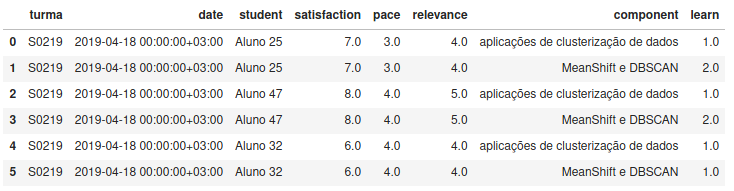
\includegraphics[width=\textwidth]{tidy-sample}
	\label{tab:dataset-raw}
\end{table}

Note que as duas primeiras linhas representam as respostas do ``Aluno 25'' ao formulário aplicado na aula de 18/abr/2019 da turma S2019. Nessa aula dois tópicos foram abordados: ``aplicações de clusterização de dados'' e ``MeanShift e DBSCAN''. No primeiro deles a aprendizagem foi de 1 unidade (última coluna) e, no segundo, de 2 unidades.

Em vista de cada formulário poder apresentar até quatro tópicos (dois neste exemplo), as informações de satisfação (\foreign{satisfaction}), ritmo (\foreign{pace}) e relevância (\foreign{relevance}) estão duplicados. Isso significa que, ao analisarmos essas variáveis, precisamos remover essas duplicidades.
Fizemos isso através de uma amostragem que selecionava, aleatoriamente, \emph{uma} linha para cada tupla (curso, turma, aula, aluno).
Por exemplo, se selecionássemos a primeira linha, certamente ignoraríamos a segunda linha.

Esse arquivo foi posteriormente transformado:
\begin{compactitem}
	\item Criamos uma coluna para identificar o curso (\foreign{course}), com valores DA ou DS, a partir da turma: aquelas que iniciam com ``A'' são de DA; as com ``S'', são DS.
	
	\item A turma foi trocada por um valor numérico sequencial arbitrário.
	
	\item As colunas de satisfação, ritmo e relevância foram normalizadas no intervalo $[0,10]$, apenas por simplicidade.

	\item Criamos a coluna \foreign{component}, que mapeia o tópico para uma hierarquia \foreign{ad-hoc} de componentes de cada curso.
	Por exemplo, o tópico ``Construção e execução de queries'' foi mapeado para o componente ``SQL/\textbf{Ferramenta}'' (DA), enquanto ``ARIMA. SARIMAX e Prophet'' foi mapeado para ``Séries temporais/\textbf{Algoritmo}'' (DS).
	O mapeamento foi feito manualmente para os 985 tópicos presentes.

	\item Criamos a coluna \foreign{tool}, variável categórica booleana, para indicar se a aula contém algum componente de ferramenta.
	Isso foi feito a partir da coluna \foreign{component}: se ela contém ``Ferramenta'', então o valor dessa variável é ``verdadeiro''; se não, é ``falso'' (veja grifos no item anterior).
	
	\item Criamos a coluna \foreign{algorithm}, variável categórica booleana, para indicar se a aula contém algum componente de algoritmo.
	Isso foi feito de maneira similar ao item anterior, também a partir da coluna \foreign{component}.
\end{compactitem}

A Tabela~\ref{fig:dataset} ilustra o conjunto de dados após esse pré-processamento e já pronto para a análise.

\begin{table}
	\centering
	\caption{O conjunto de dados, pronto para a análise.}
	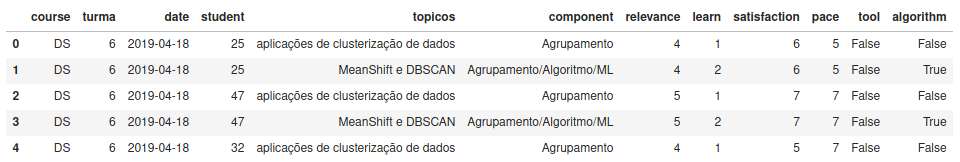
\includegraphics[width=\textwidth]{tidy-sample-2}
	\label{fig:dataset}
\end{table}